\chapter{Zielsetzung}
Bei dem Projekt "`Sportangebot der HTW"' ging es darum, einen Beratungsassistenten zu erstellen. Hierbei handelt es sich um ein Softwareprodukt, bei dem der sportinteressierte Benutzer Auswahlkriterien festlegen kann, woraufhin das Produkt geeignete Sportarten vorschlägt, die vom Hochschulsport der HTW angeboten werden.

\section{Szenarien}
Als Testfall wurden zwei Szenarien aufgestellt. Diese Szenarien gehen davon aus, dass das Produkt einen menschlichen Berater ersetzen soll. Dies bedeutet, dass die Szenarien aus einzelnen Fragen bestehen, die der Berater dem Studenten stellt, um die Sportarten einzugrenzen. Dies bedeutet, dass nach jeder Frage einige Sportarten herausgefiltert werden. Weiterhin sind Sprünge im Szenario vorgesehen. Dies bedeutet, dass je nach Antwort auf eine Frage, auf eine bestimmte andere Frage gesprungen wird.

Weiterhin wurden bei den Szenarien bereits Überlegungen getroffen, ob die Fragen durch die Ontologie oder durch die Datenbank abgehandelt werden sollen. Dabei wurde als Grundregel angewandt, dass jenes Wissen durch die Ontologie abgebildet wird, welches auch der Berater wissen würde. Z.B. ist Fußball ein Teamsport? Auf der anderen Seite wurden jene Fakten die der Berater ebenfalls nachschlagen würde in der Datenbank gespeichert. Z.B. an welchen Tagen und zu welchen Uhrzeiten ist das Fußballtraining?

Die folgenden Abbildungen (\ref{fig:Szenario 1} und \ref{fig:Szenario 2}) stellen die Szenarien dar, wie sie das Team zum Zeitpunkt des ersten Meilensteins ausgearbeitet hat.

\begin{capfigure}[Szenario 1]
	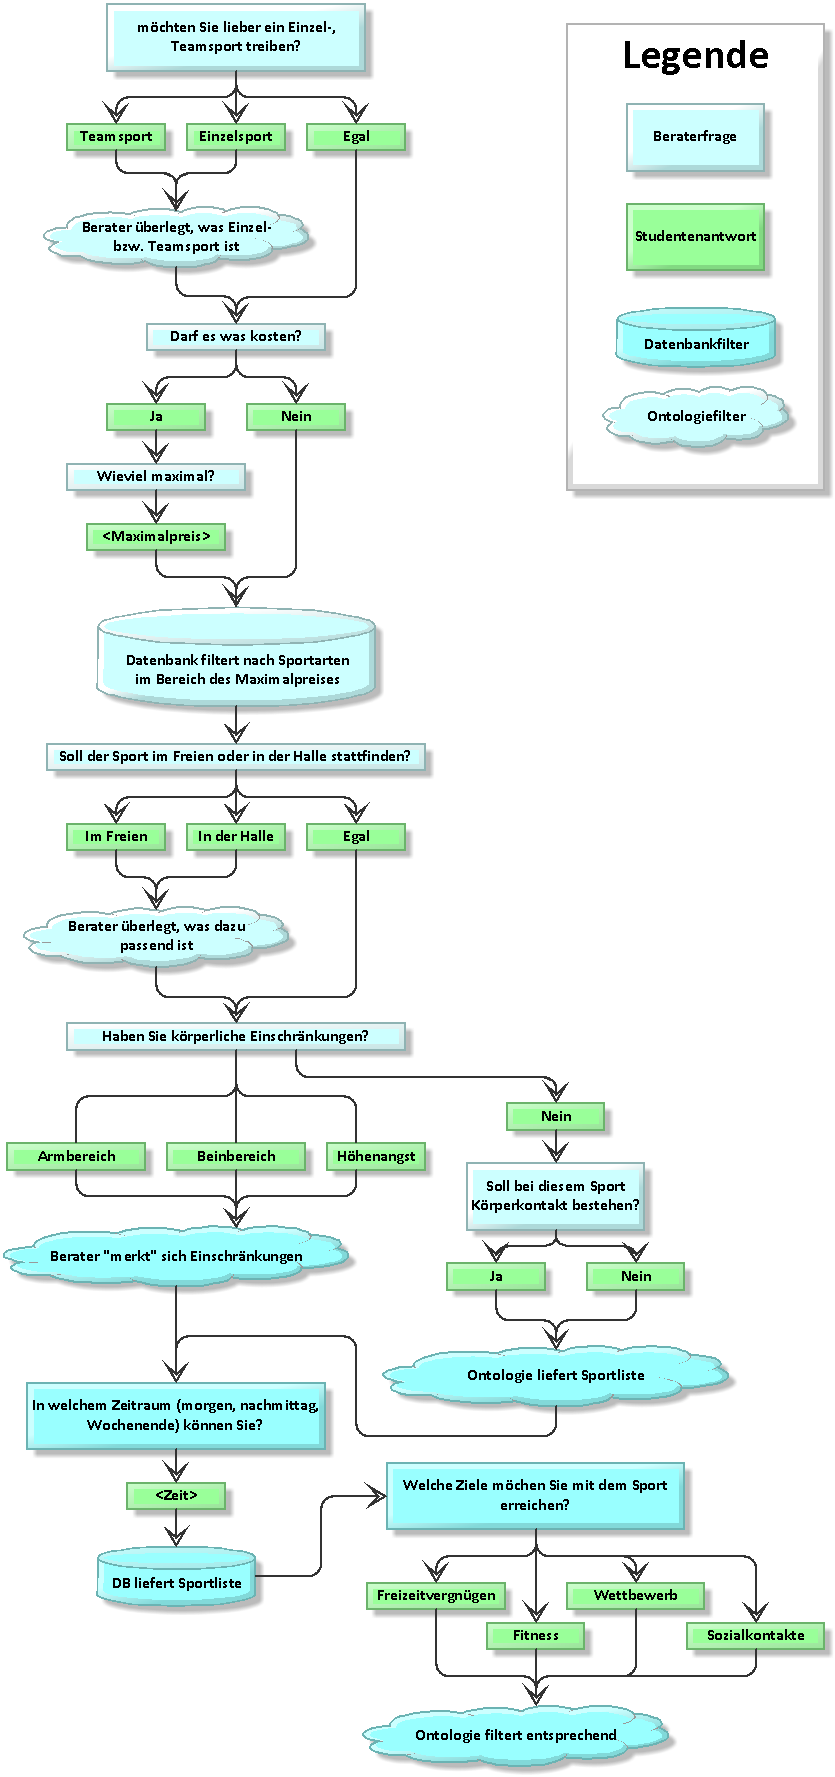
\includegraphics[width=100mm]{images/szenario1.png}
\end{capfigure}

\begin{capfigure}[Szenario 2]
	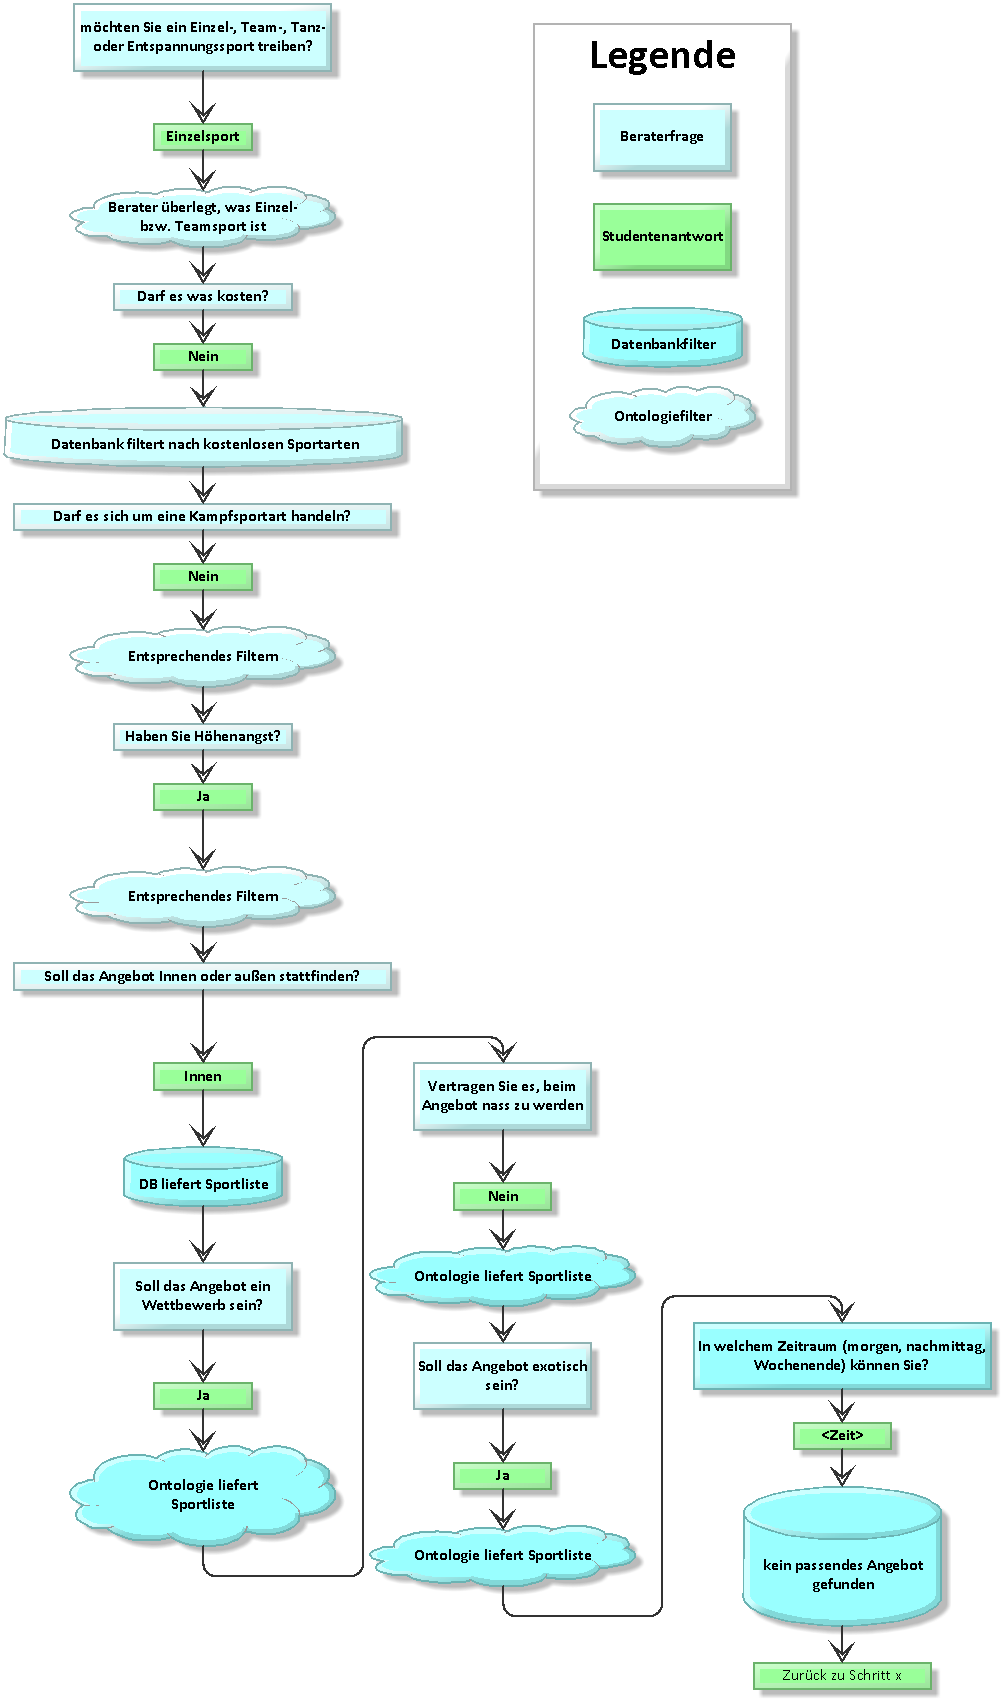
\includegraphics[width=100mm]{images/szenario2.png}
\end{capfigure}
